\chapter{EPS mission engineering flows}
\label{appendix:eps-mission-flows}

\begingroup
\renewcommand{\baselinestretch}{1.0}
\small
Short verb phrases name activities. Other rectangles identify incoming context and phase handoffs. Diamonds denote review acceptance. Solid arrows carry engineering information. Dotted arrows return findings. Dashed arrows carry authorization. Exchange labels identify the main information passed between activities. The accumulated review basis remains an input to subsequent work. The designated review authority controls acceptance and its conditions. Activities recur across phases under change control.
\par
\endgroup

\begingroup
\captionsetup{font=small,skip=4pt}
\begin{figure}[H]
    \centering
    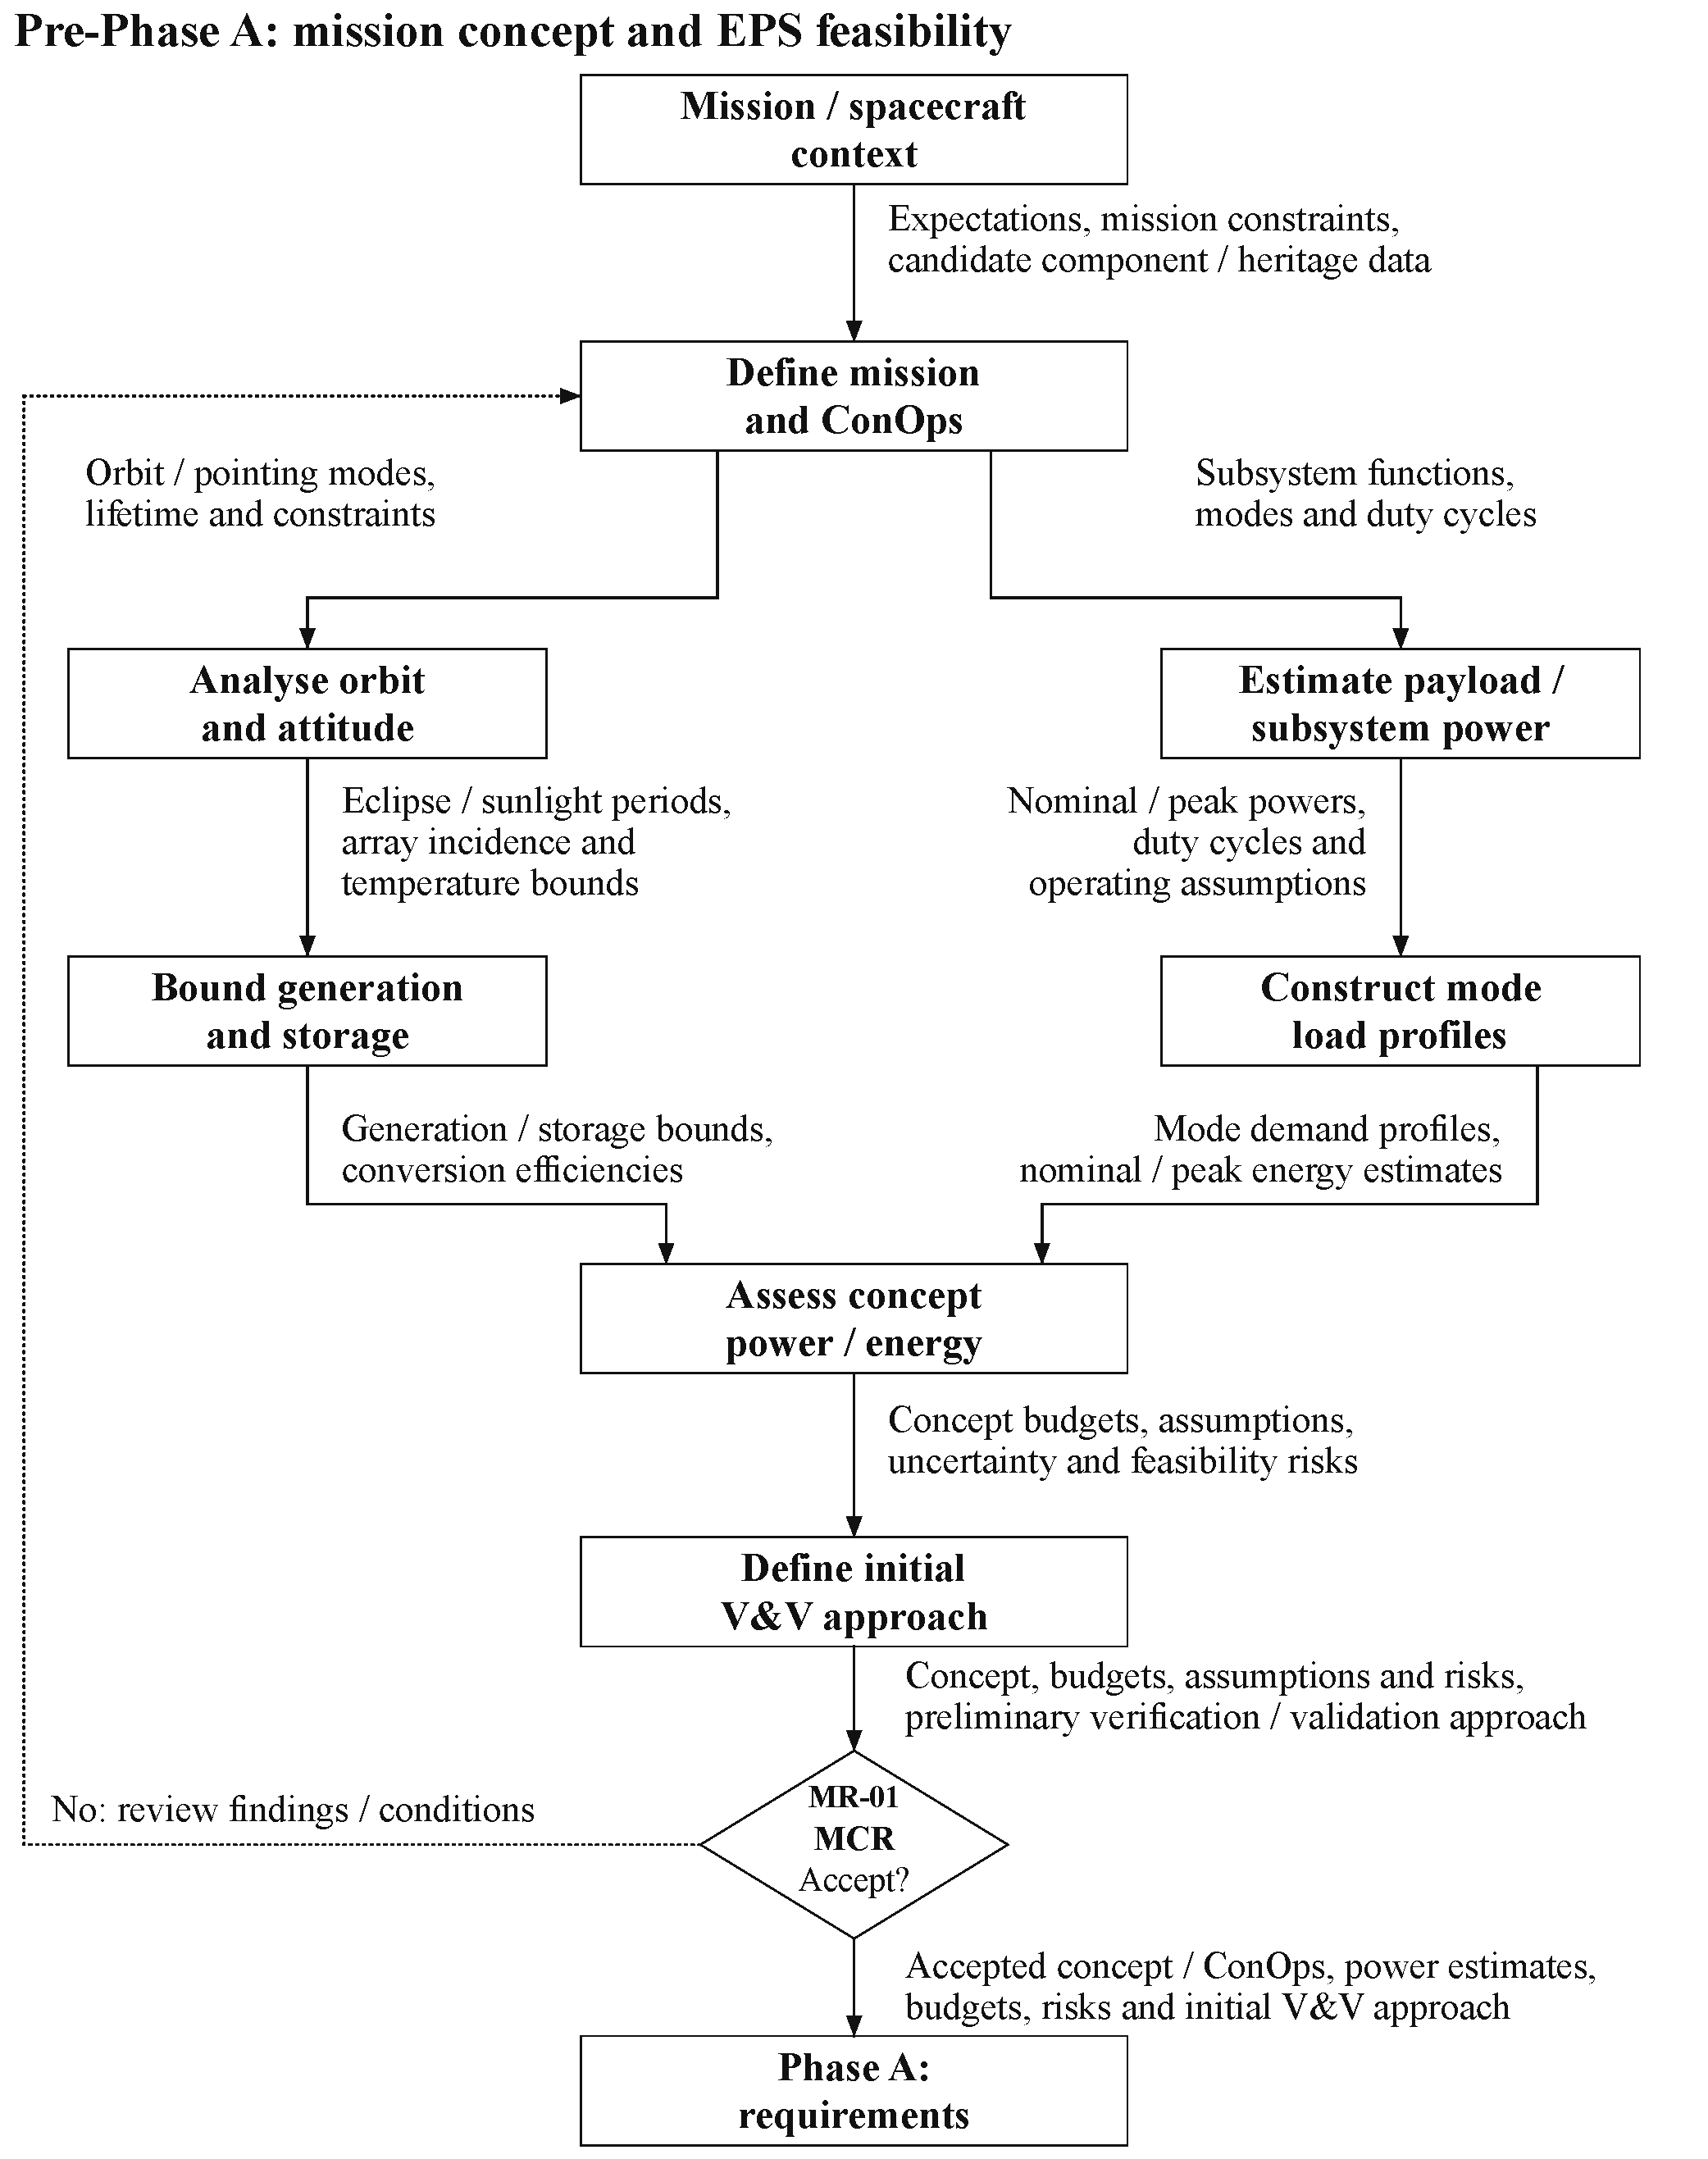
\includegraphics[width=\linewidth,height=\dimexpr\textheight-85pt\relax,keepaspectratio]{fig/eps-mission-requirements-flow-pre-a.pdf}
    \caption[Pre-Phase A activity flow for MR-01.]{Pre-Phase A activity flow for MR-01. Sourced demand estimates and generation and storage bounds support concept feasibility. Orbit and attitude analysis supplies illumination constraints. This is a proposed decomposition of NASA concept studies \citep[Secs.~2.3 and~3.3]{nasa2016systems} and EPS mission analysis \citep[Secs.~2--3]{handpicked-0003}.}
    \label{fig:eps-mission-pre-a}
\end{figure}
\clearpage

\begin{figure}[H]
    \centering
    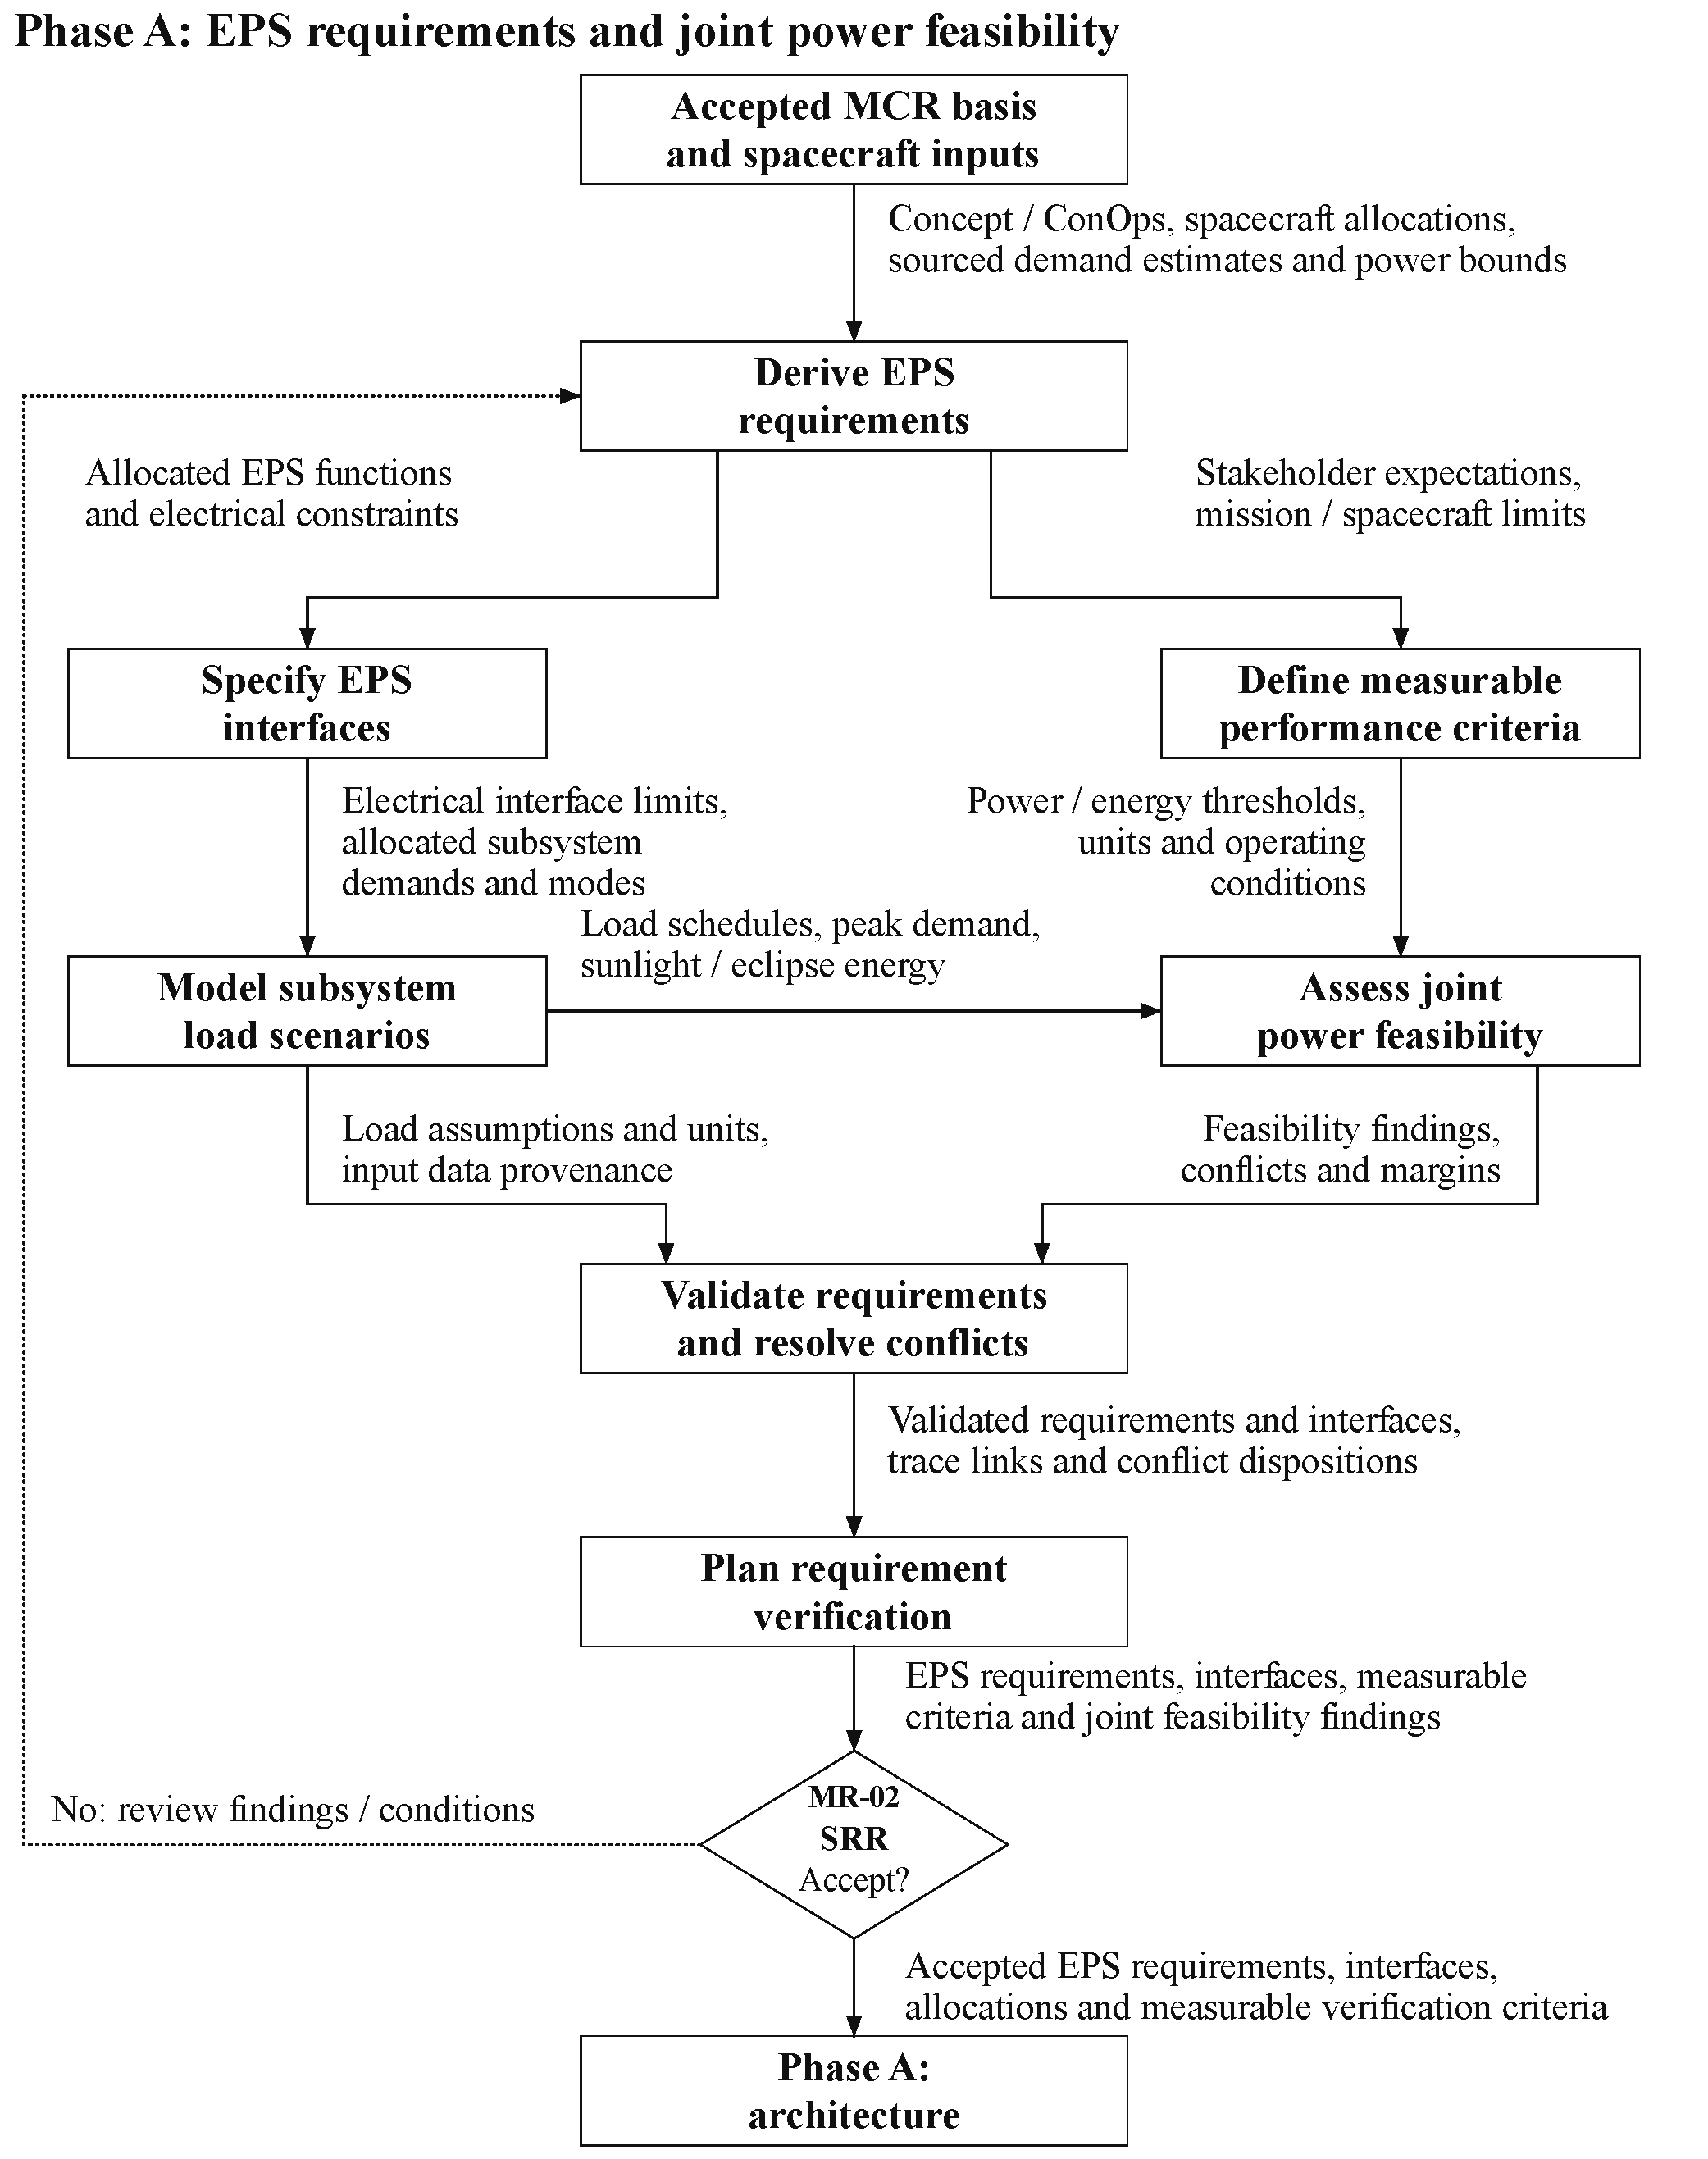
\includegraphics[width=\linewidth,height=\dimexpr\textheight-85pt\relax,keepaspectratio]{fig/eps-mission-requirements-flow-phase-a-requirements.pdf}
    \caption[Phase A requirements activity flow for MR-02.]{Phase A requirements activity flow for MR-02. Joint feasibility checks assess EPS requirements together with the power implications of mission and subsystem requirements before SRR. NASA requirements validation \citep[Secs.~3.4 and~4.2]{nasa2016systems} is combined with EPS demand and duty cycle analysis \citep[Secs.~2--3]{handpicked-0003}.}
    \label{fig:eps-mission-a-requirements}
\end{figure}
\clearpage

\begin{figure}[H]
    \centering
    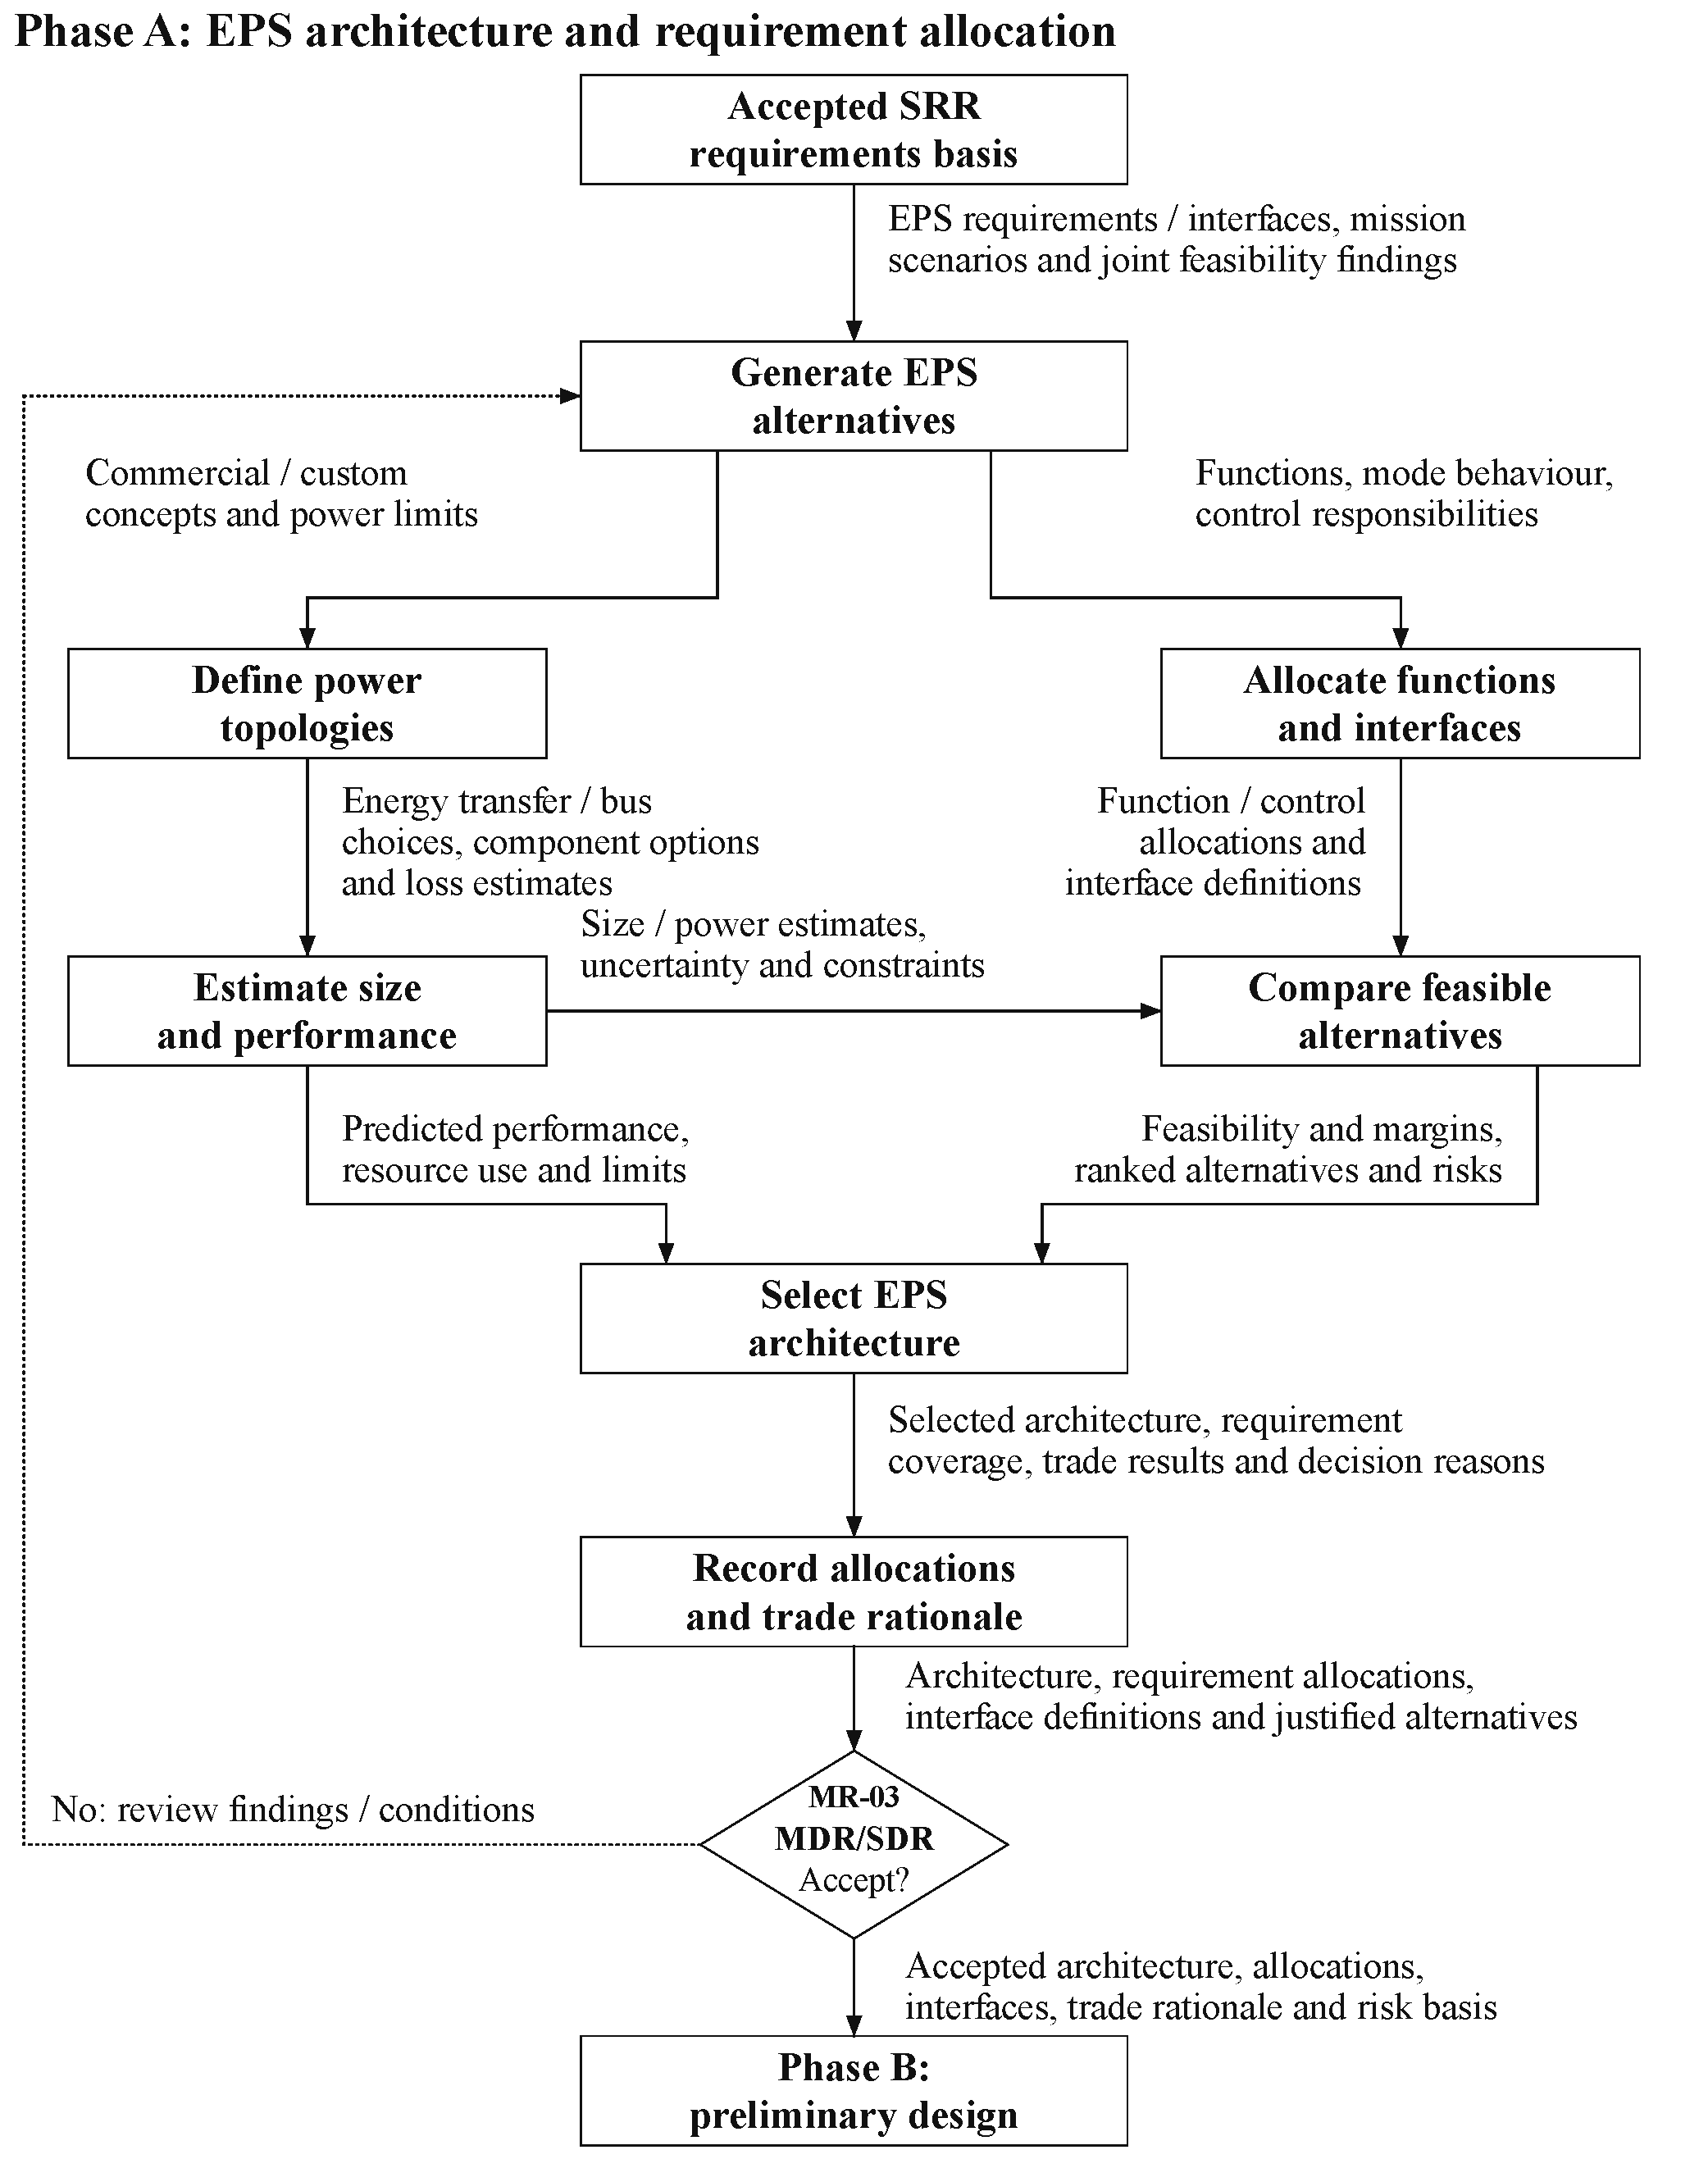
\includegraphics[width=\linewidth,height=\dimexpr\textheight-85pt\relax,keepaspectratio]{fig/eps-mission-requirements-flow-phase-a-architecture.pdf}
    \caption[Phase A architecture activity flow for MR-03.]{Phase A architecture activity flow for MR-03. Concept estimates support alternative comparison and requirement allocation at MDR/SDR \citep[Sec.~3.4, Table~6.7-1]{nasa2016systems}. Commercial and custom designs, power topology, regulation and distribution supply the EPS alternatives \citep[Sec.~4]{handpicked-0003}. Detailed preliminary sizing follows in Phase B.}
    \label{fig:eps-mission-a-architecture}
\end{figure}
\clearpage

\begin{figure}[H]
    \centering
    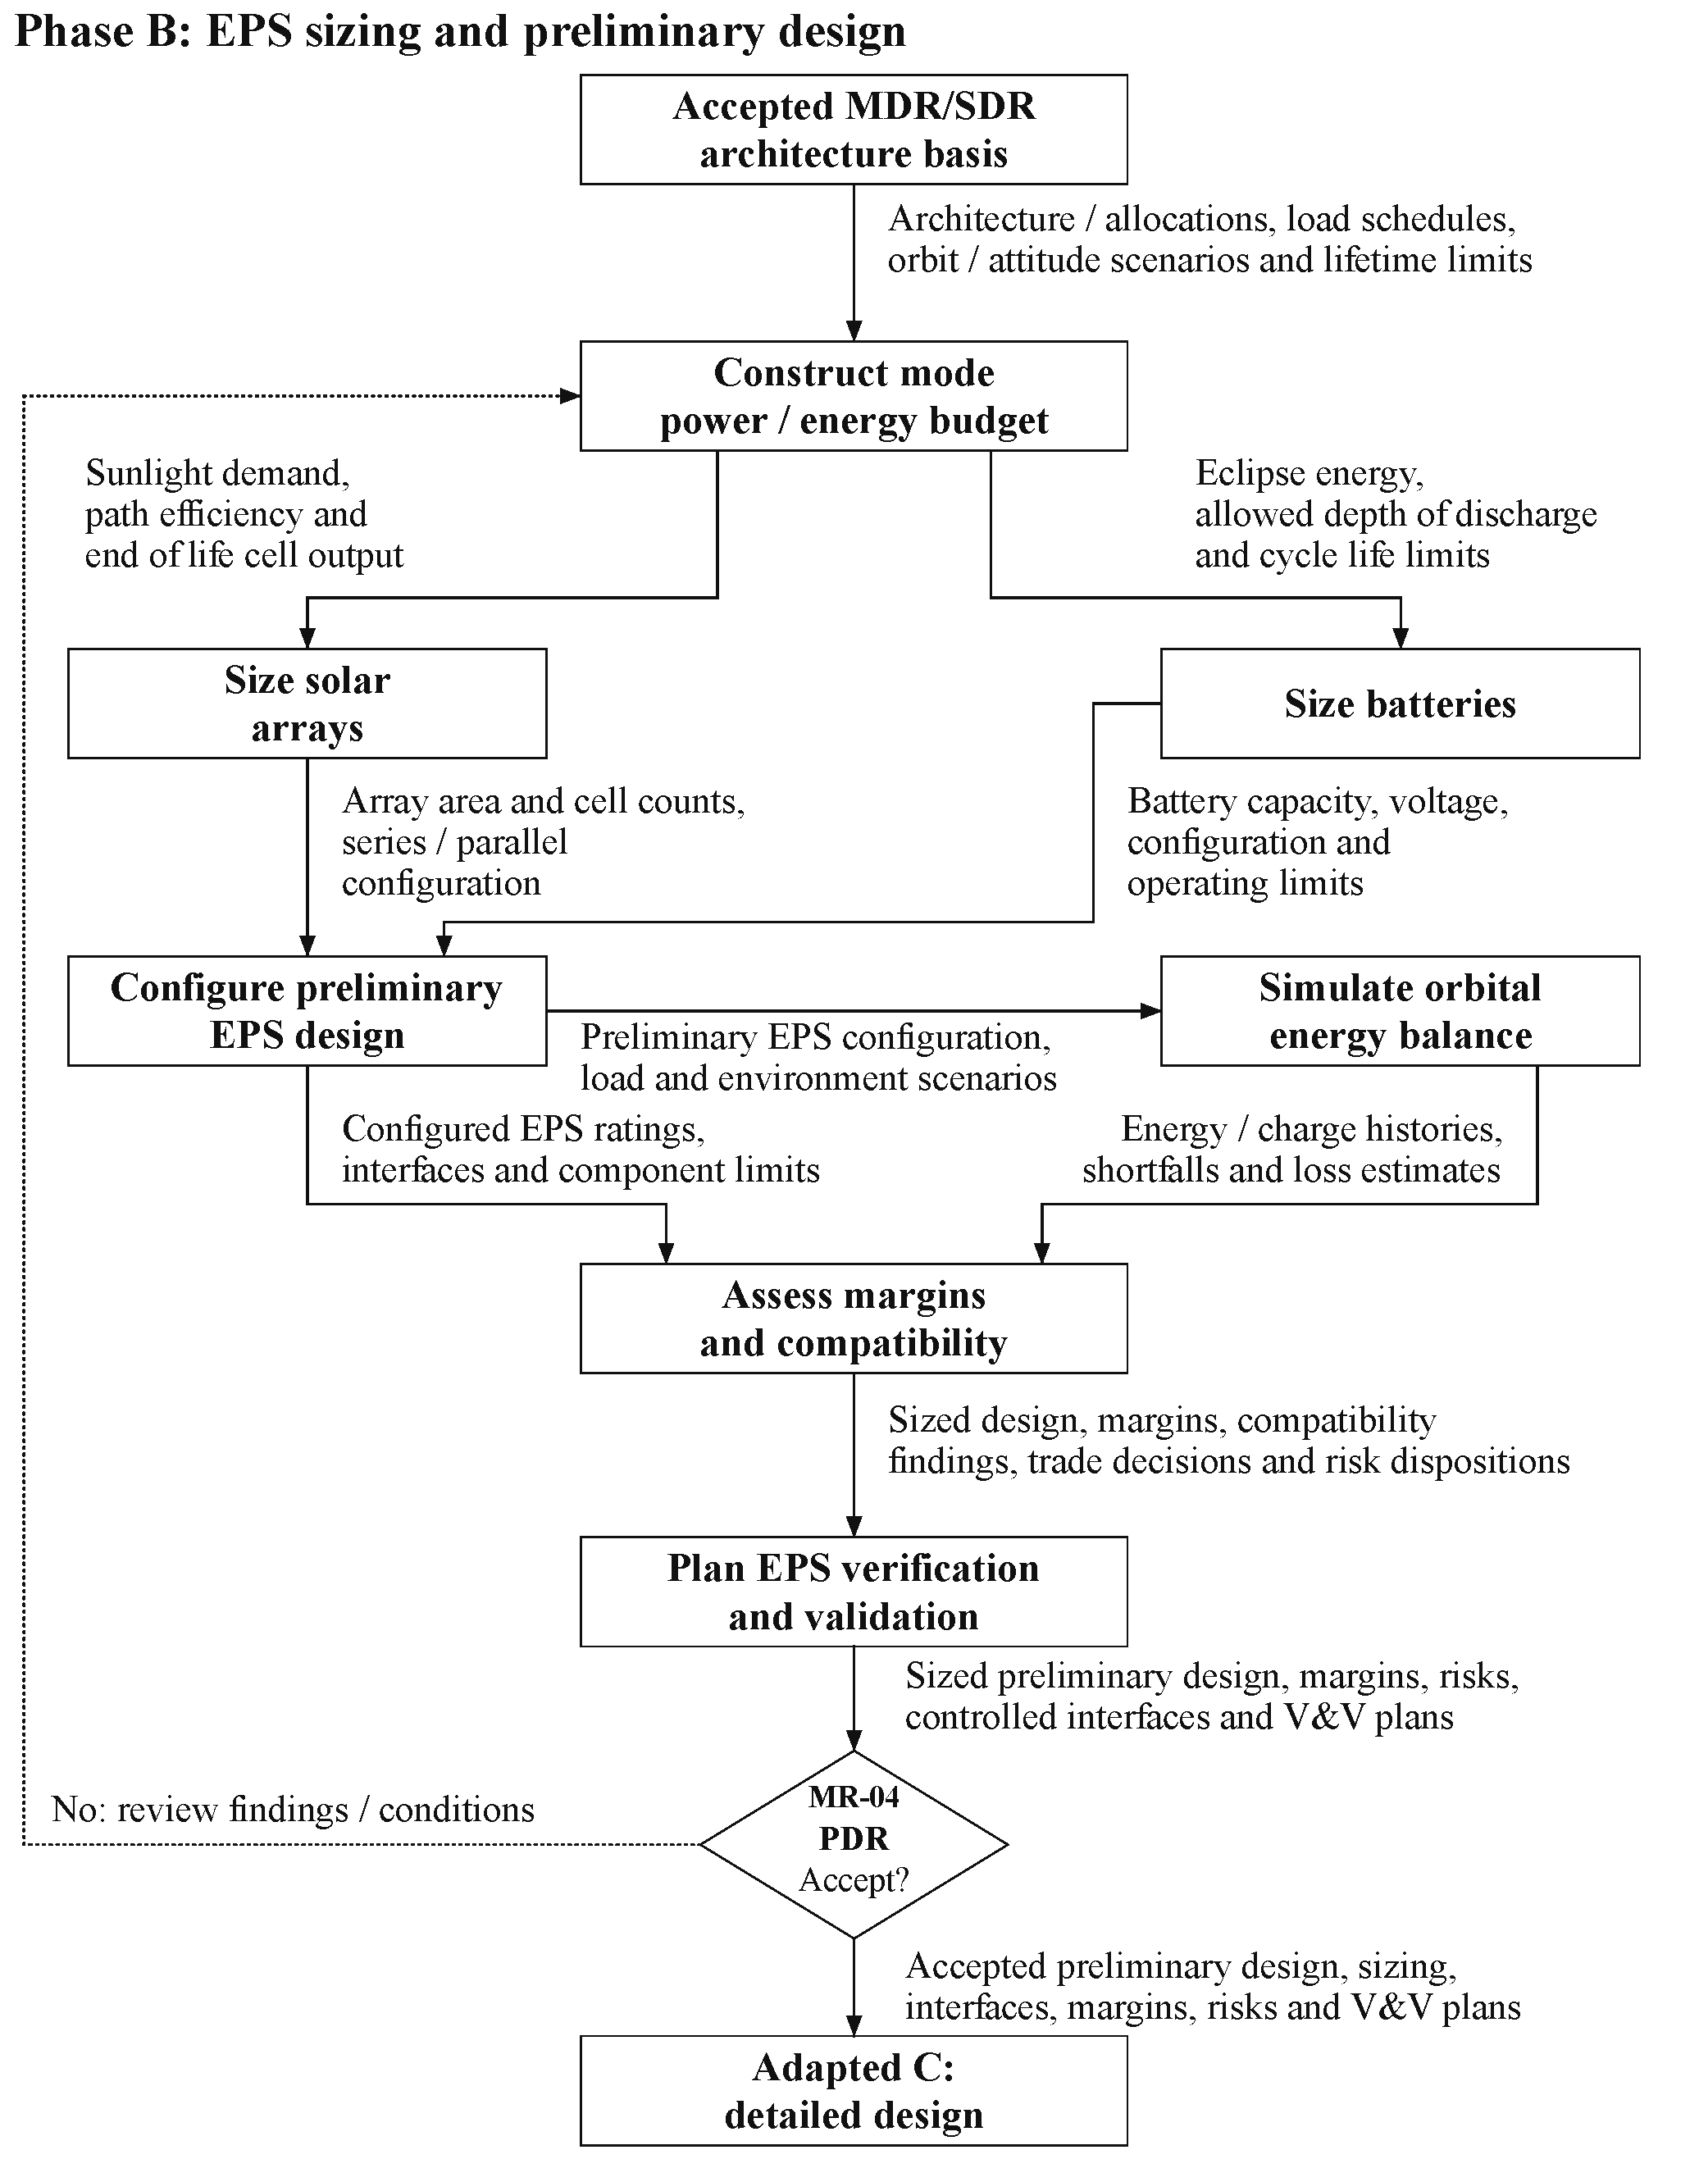
\includegraphics[width=\linewidth,height=\dimexpr\textheight-85pt\relax,keepaspectratio]{fig/eps-mission-requirements-flow-phase-b.pdf}
    \caption[Phase B activity flow for MR-04.]{Phase B activity flow for MR-04. Losses, degradation and discharge limits inform array and battery sizing. Orbital energy histories support design compatibility and margin assessment. The PDR purpose follows NASA \citep[Sec.~3.5, Table~6.7-1]{nasa2016systems}. Sizing and orbital assessment follow EPS activities from El Hachimi et al. \citep[Secs.~3 and~6.2]{handpicked-0003}.}
    \label{fig:eps-mission-b}
\end{figure}
\clearpage

\begin{figure}[H]
    \centering
    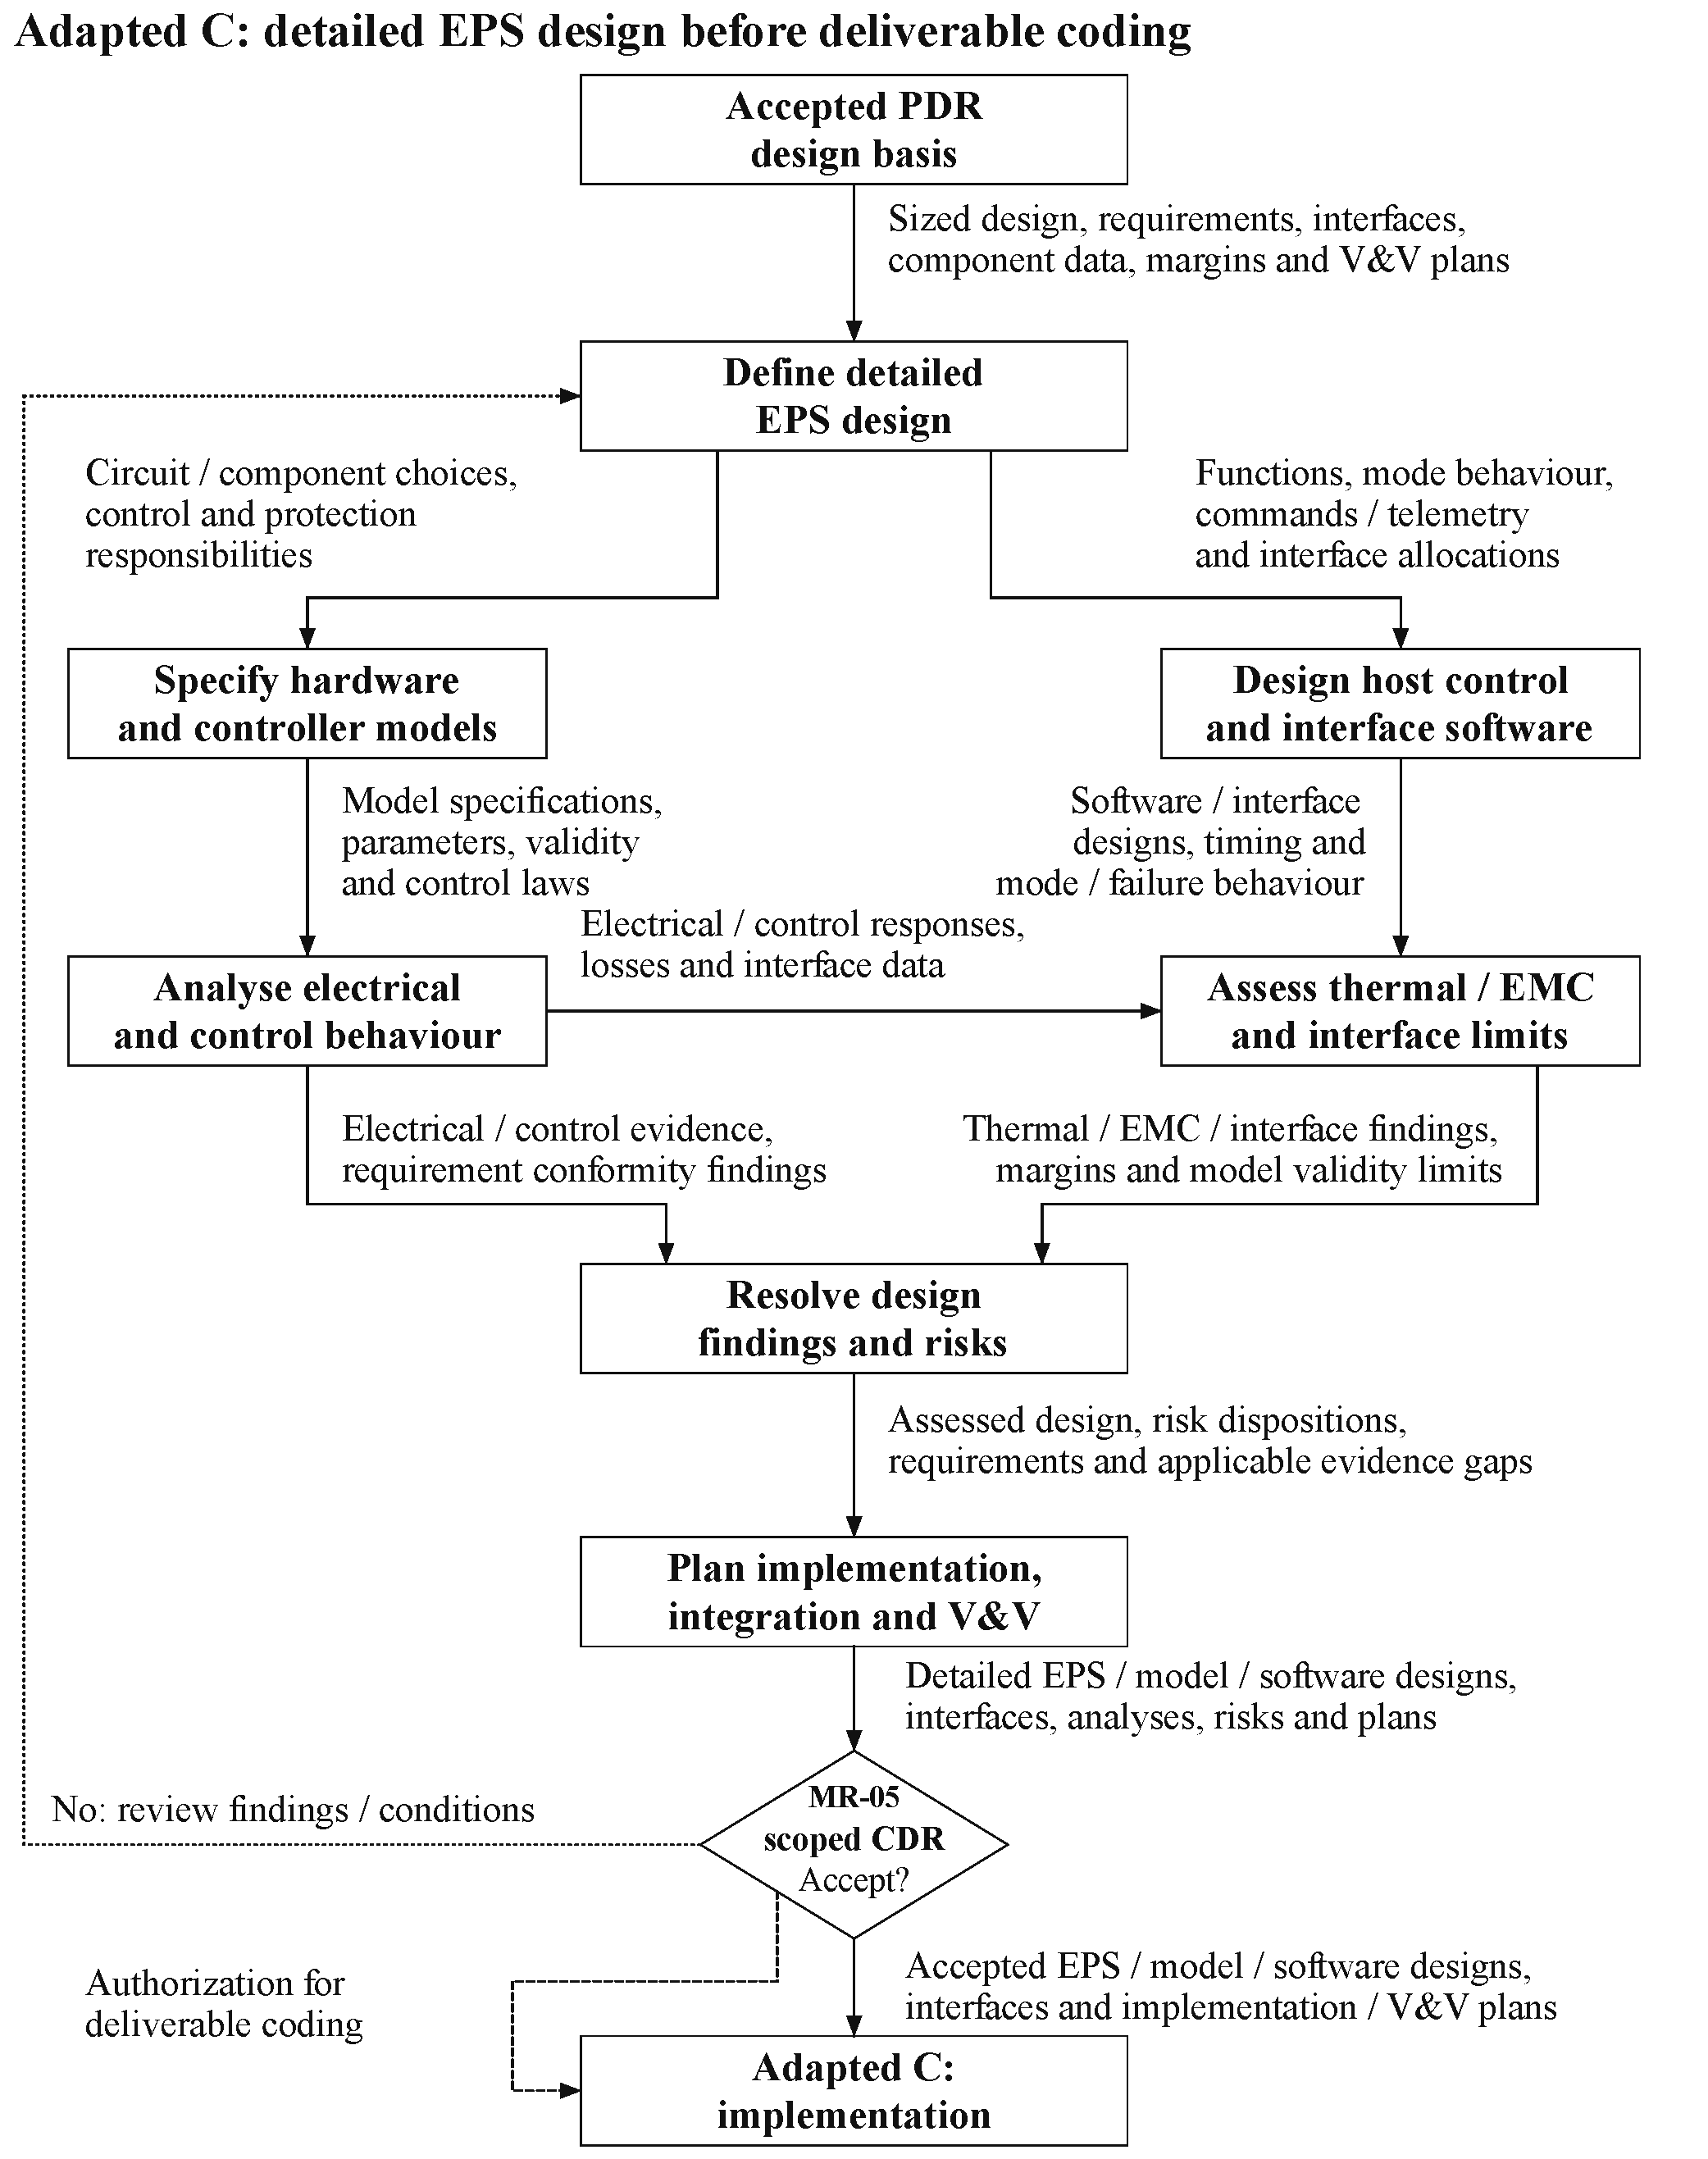
\includegraphics[width=\linewidth,height=\dimexpr\textheight-85pt\relax,keepaspectratio]{fig/eps-mission-requirements-flow-phase-c-design.pdf}
    \caption[Adapted Phase C detailed design flow for MR-05.]{Adapted Phase C detailed design flow for MR-05. Earlier models can support design analyses. Scoped CDR accepts the detailed EPS design and authorizes deliverable coding \citep[Sec.~3.6, Table~6.7-1]{nasa2016systems}. Electrical, protection, thermal and EMC activities follow the EPS design study \citep[Secs.~4 and~7]{handpicked-0003}. Hardware and controller modeling support this scoped assessment \citep[Sec.~2]{review-0573}.}
    \label{fig:eps-mission-c-design}
\end{figure}
\clearpage

\begin{figure}[H]
    \centering
    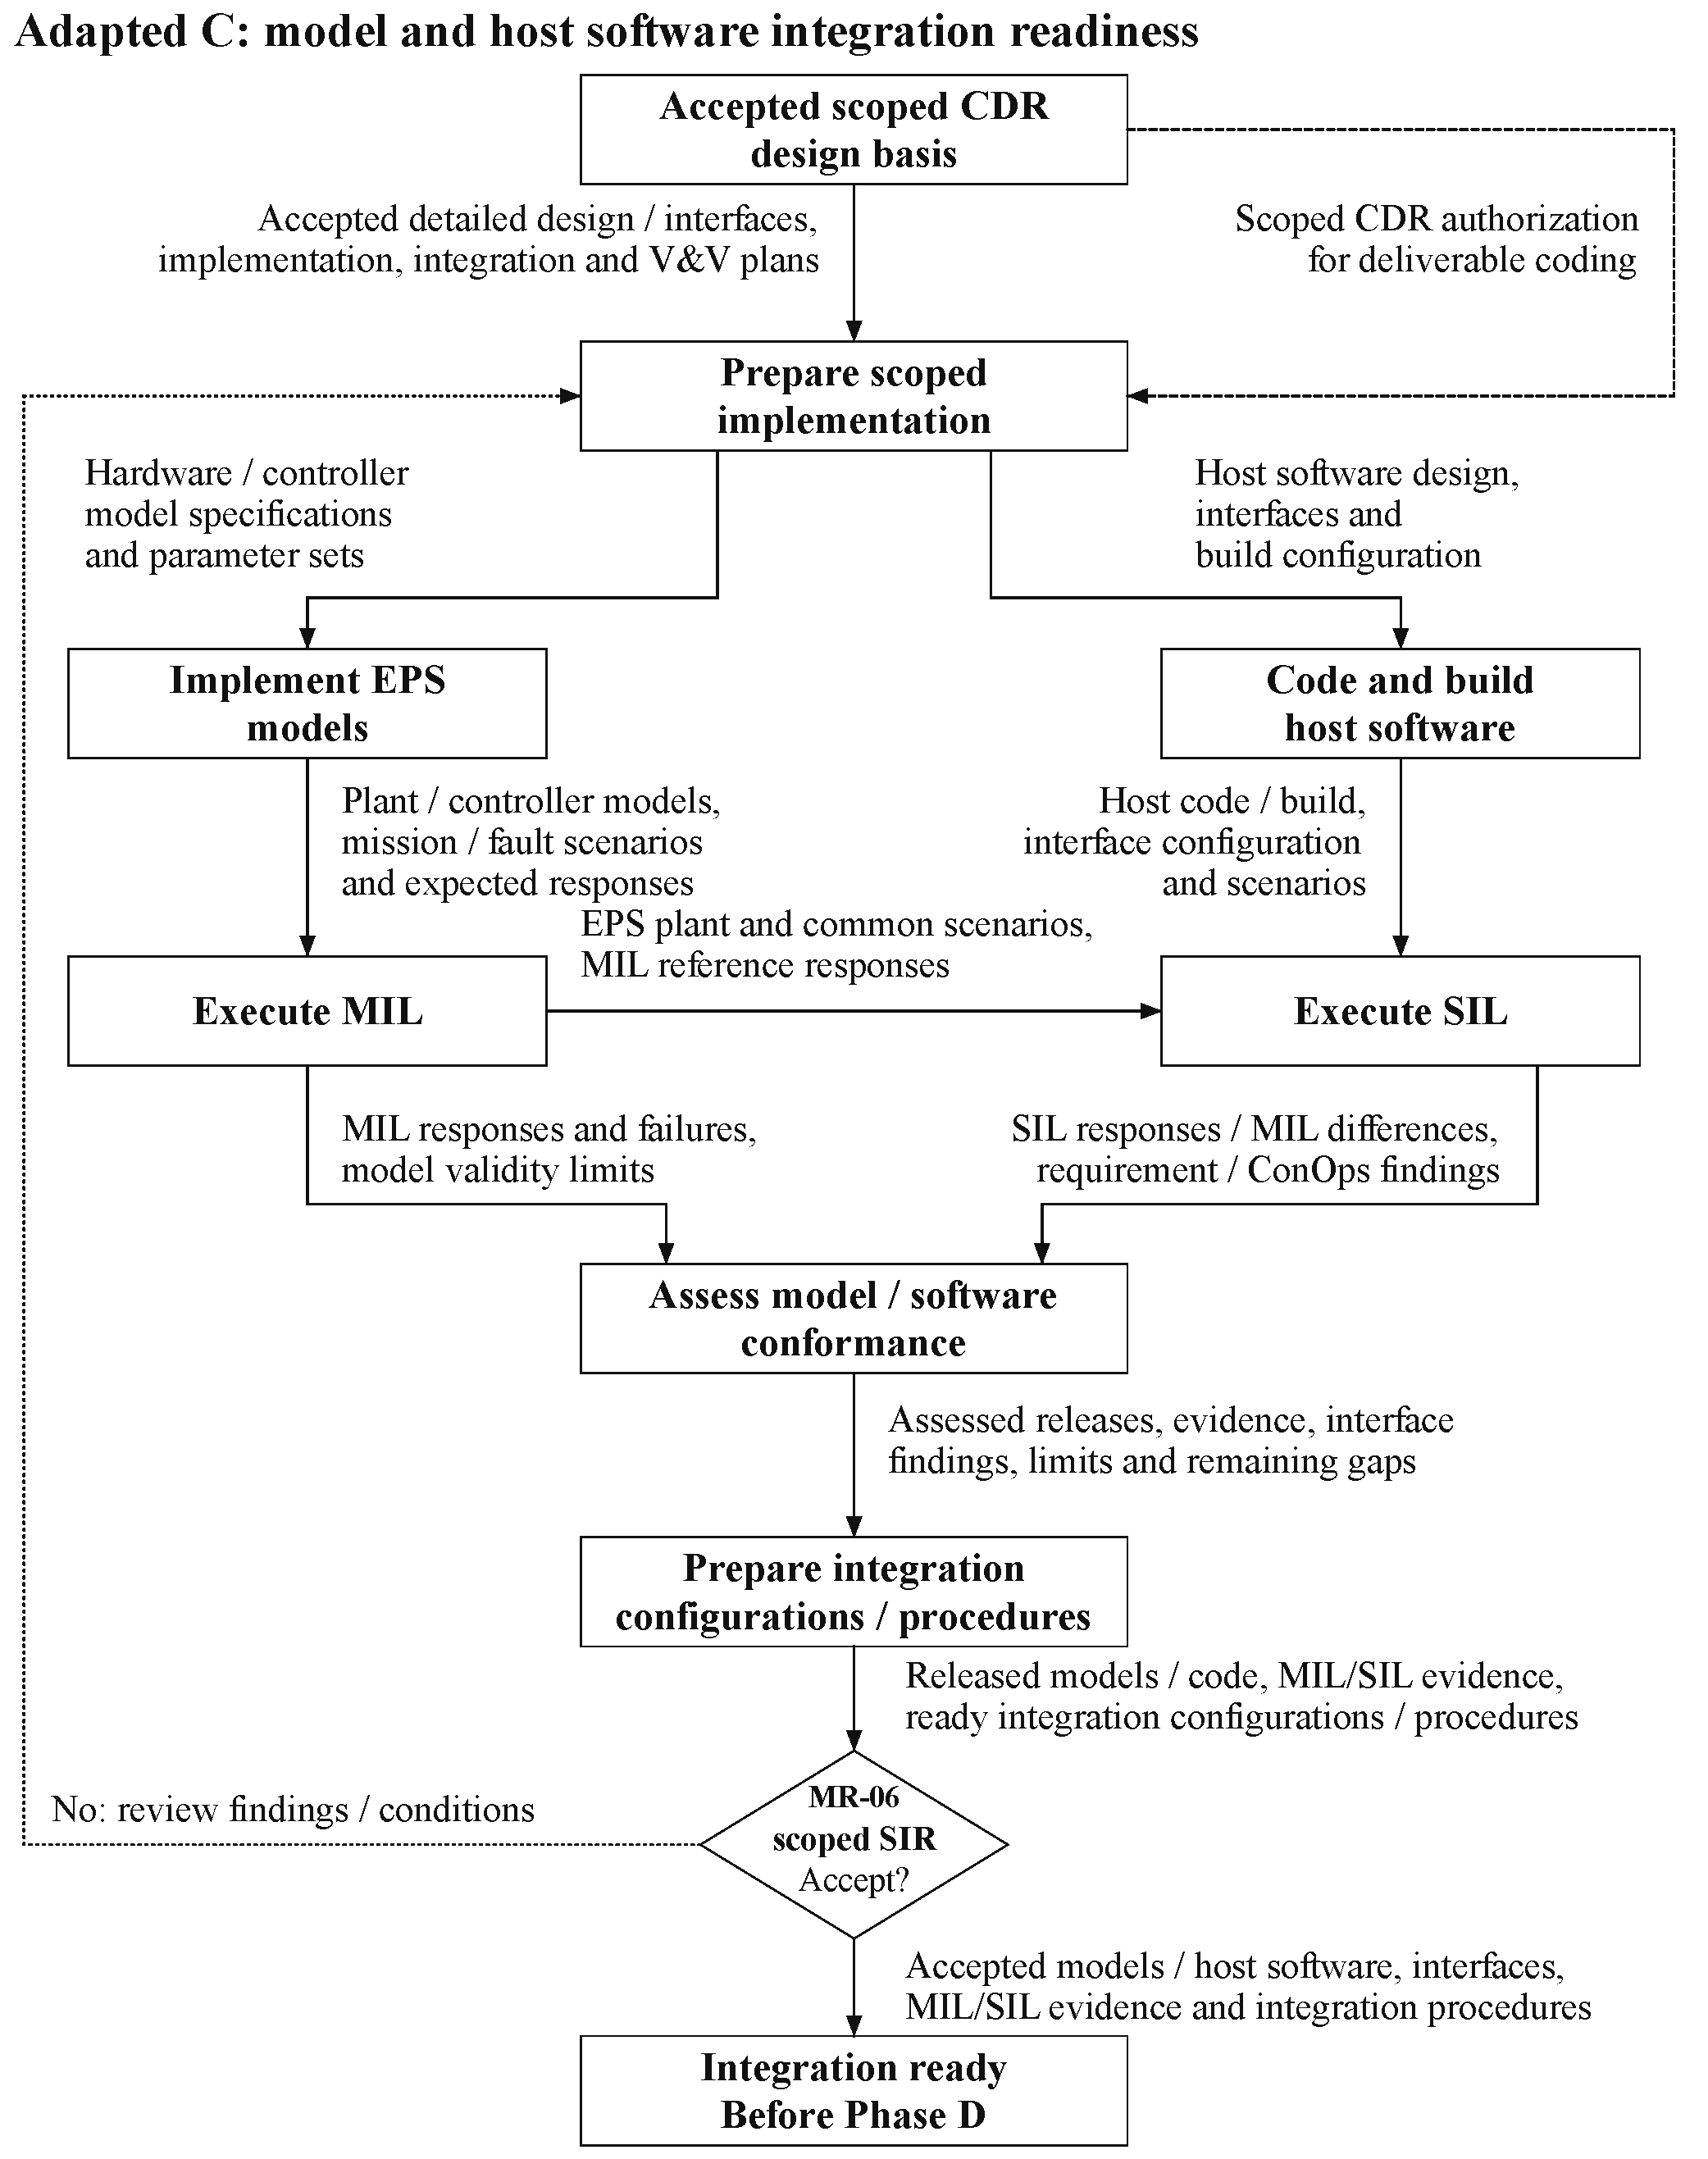
\includegraphics[width=\linewidth,height=\dimexpr\textheight-85pt\relax,keepaspectratio]{fig/eps-mission-requirements-flow-phase-c-readiness.pdf}
    \caption[Adapted Phase C integration readiness flow for MR-06.]{Adapted Phase C integration readiness flow for MR-06. Scoped CDR authorization precedes deliverable coding. MIL and SIL assess the declared models and host software. EPS scenarios cover charging, protection, recovery, changing loads and telemetry \citep[Secs.~8.1.5--8.1.7]{handpicked-0003}. Scoped SIR retains NASA's integration readiness purpose \citep[Sec.~3.6, Table~6.7-1]{nasa2016systems}. The scope ends before Phase D. Physical qualification is excluded.}
    \label{fig:eps-mission-c-readiness}
\end{figure}
\endgroup
\clearpage
